\documentclass{article}

\usepackage{graphicx}
\usepackage{tikz}
\usepackage{tikzsymbols}
\usetikzlibrary{calc,patterns,shapes.geometric}
\pagestyle{empty}
\usepackage[margin=0pt]{geometry}
\geometry{papersize={14in,12in}}

\def\centerarc[#1](#2)(#3:#4:#5){\draw[#1] ($(#2)+({#5*cos(#3)},{#5*sin(#3)})$) arc (#3:#4:#5);}

\begin{document}
	\begin{figure}
		\centering
		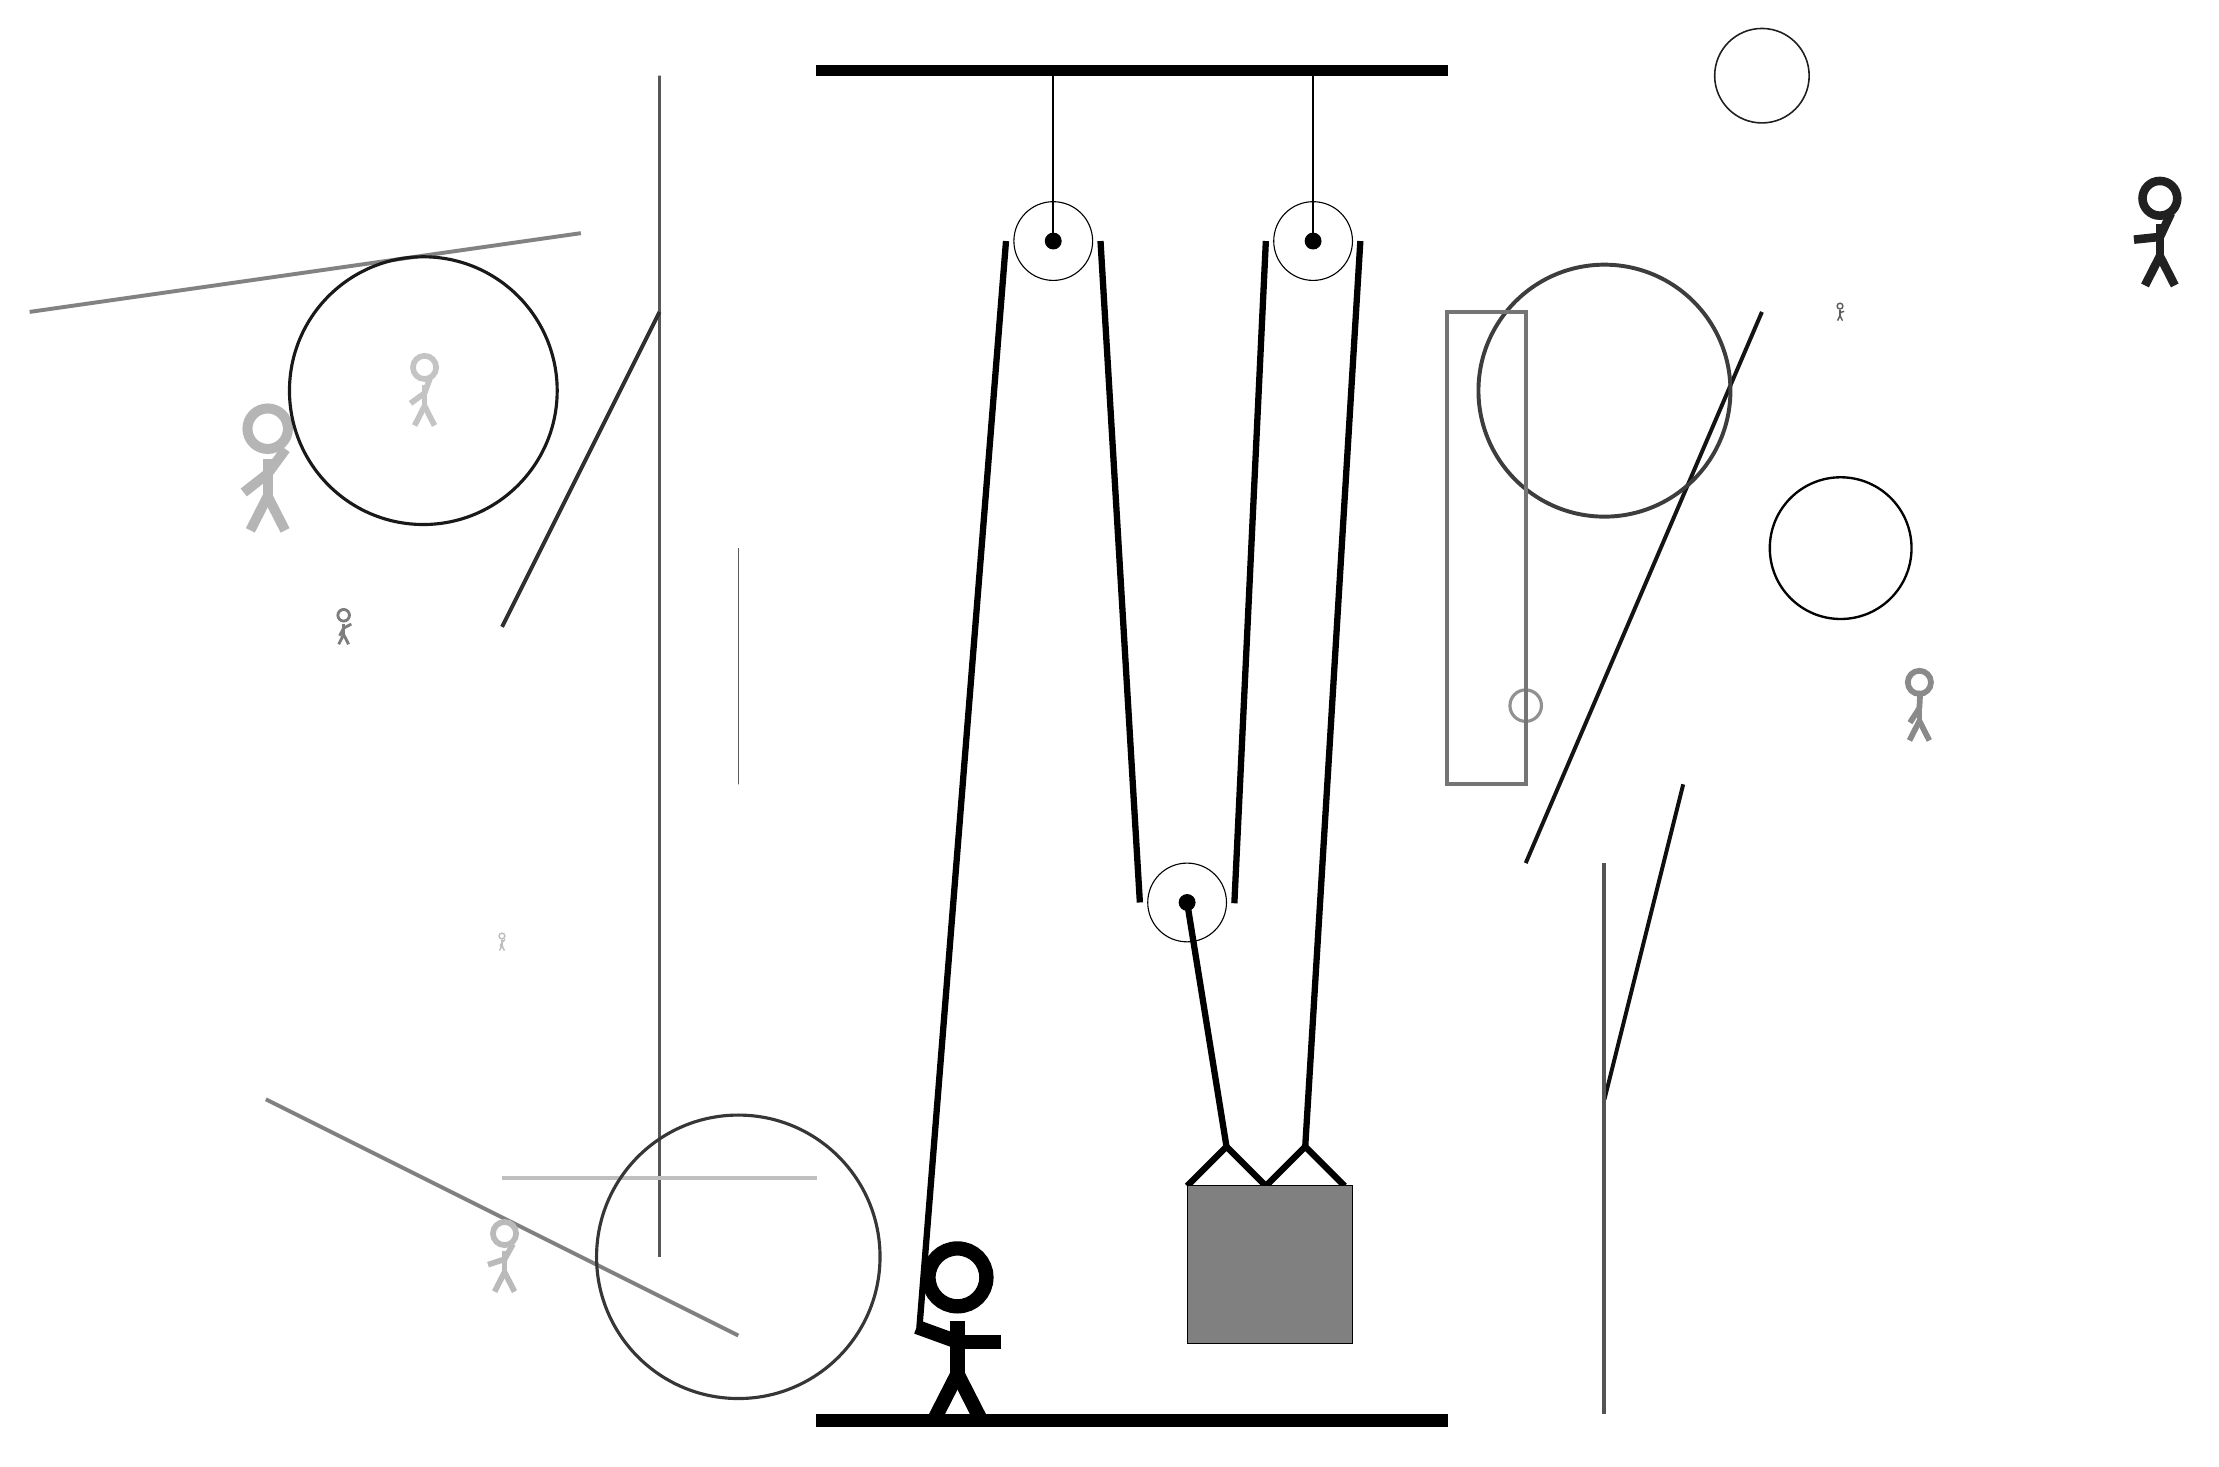
\begin{tikzpicture}
			%%%%% START %%%%%
			
			\draw[fill=black] (-2, 14) rectangle (6, 14.125);
			
			\draw (1, 11.9) circle (0.5);
			\draw[fill=black] (1, 11.9) circle (0.1);
			\draw[thick] (1, 11.9) -- (1, 14);
			
			\draw (4.3, 11.9) circle (0.5);
			\draw[fill=black] (4.3, 11.9) circle (0.1);
			\draw[thick] (4.3, 11.9) -- (4.3, 14);
			
			\draw [line width=0.3mm, color=black!99](11, 8) circle (0.9);
			
			\node[line width=0.3mm, color=black!23] at (-7, 10) {\Strichmaxerl[4][36][70]};
			\draw[line width=0.3mm, color=black!66] (-4, -1) rectangle (-4, 14);
			\draw [line width=0.2mm, color=black!88](10, 14) circle (0.6);
			\draw[line width=0.5mm, color=black!94](9, 5) -- (8, 1);
			
			\draw[line width=0.5mm, color=black!49](-5, 12) -- (-12, 11);
			
			\node[line width=0.5mm, color=black!29] at (-9, 9) {\Strichmaxerl[7][38][54]};
			
			\draw[line width=0.5mm, color=black!81](-4, 11) -- (-6, 7);
			\draw[line width=0.5mm, color=black!25](-2, 0) -- (-6, 0);
			
			\node[line width=0.6mm, color=black!87] at (15, 12) {\Strichmaxerl[6][6][65]};
			\draw[line width=0.2mm, color=black!64] (-3, 5) rectangle (-3, 8);
			
			\draw [line width=0.4mm, color=black!90](-7, 10) circle (1.7);
			\node[line width=0.6mm, color=black!46] at (12, 6) {\Strichmaxerl[4][57][87]};
			
			\draw[line width=0.5mm, color=black!67](8, 4) -- (8, -3);
			\draw [line width=0.4mm, color=black!43](7, 6) circle (0.2);
			\draw[line width=0.5mm, color=black!50](-3, -2) -- (-9, 1);
			
			\node[line width=0.4mm, color=black!63] at (11, 11) {\Strichmaxerl[1][84][16]};
			\draw [line width=0.4mm, color=black!79](-3, -1) circle (1.8);
			\node[line width=0.6mm, color=black!27] at (-6, -1) {\Strichmaxerl[4][18][61]};
			
			\node[line width=0.7mm, color=black!51] at (-8, 7) {\Strichmaxerl[2][62][28]};
			\node[line width=0.4mm, color=black!26] at (-6, 3) {\Strichmaxerl[1][64][44]};
			\draw[line width=0.5mm, color=black!92](10, 11) -- (7, 4);
			
			\draw[line width=0.3mm, color=black!21] (7, 6) rectangle (7, 11);
			\draw [line width=0.5mm, color=black!76](8, 10) circle (1.6);
			\draw[line width=0.5mm, color=black!54] (7, 11) rectangle (6, 5);
			
			
			\draw (2.7, 3.5) circle (0.5);
			\draw[fill=black] (2.7, 3.5) circle (0.1);
			
			\draw[line width=0.8mm]  (2.7, -0.1) -- (3.2, 0.4) -- (3.7, -0.1) -- (4.2, 0.4) -- (4.7, -0.1);
			\draw[fill=black!50] (2.7, -0.1) rectangle (4.8, -2.1);
			
			\draw[line width=0.8mm](-0.7, -1.9) -- (0.4, 11.9);
			\centerarc[line width=0.8mm](1, 11.9)(0:180:0.6);
			\draw[line width=0.8mm](1.6, 11.9) -- (2.1, 3.5);
			\centerarc[line width=0.8mm](2.7, 3.5)(180:370:0.6);
			\draw[line width=0.8mm] (3.3, 3.49) -- (3.7, 11.9);
			\centerarc[line width=0.8mm](4.3, 11.9)(0:180:0.6);
			\draw[line width=0.8mm](4.2, 0.4) -- (4.9, 11.9);
			\draw[line width=0.8mm] (3.2, 0.4) -- (2.7, 3.5);
			
			\node at (-0.2, -2) {\Strichmaxerl[10][-20][0]};
			
			\draw[fill=black] (-2, -3) rectangle (6, -3.15);
			
			%%%%% END %%%%%
		\end{tikzpicture}
	\end{figure}	
\end{document}